% ----------------------------------------------------------
% Metodologia
% ----------------------------------------------------------
\chapter{Metodologia}
\label{chap:metodologia}

O trabalho de tese em questão trata-se, essencialmente, do desenvolvimento e testes
de um sistema de \textit{software}. Desse modo, parece desejável, do ponto de vista de
clareza, descrever a metodologia utilizada no trabalho de forma a acompanhar o ciclo
de desenvolvimento dos vários elementos de software utilizados para obter o sistema
acoplado.

\section{Visão Geral}

O sistema de \textit{software} desenvolvido tem algumas particularidades relativas à sua
implementação. Isso se deve às particularidades do problema que se pretende resolver e ao
fato não-usual de envolver duas peças de \textit{software} independentes para resolver
um problema complexo, já apresentado como um problema multi-física.

A Figura \ref{metodoetapas} apresenta uma representação gráfica do funcionamento do sistema
acoplado desenvolvido.

\begin{figure}[htb]
  \caption{Metodologia: o sistema acoplado.}
  \centering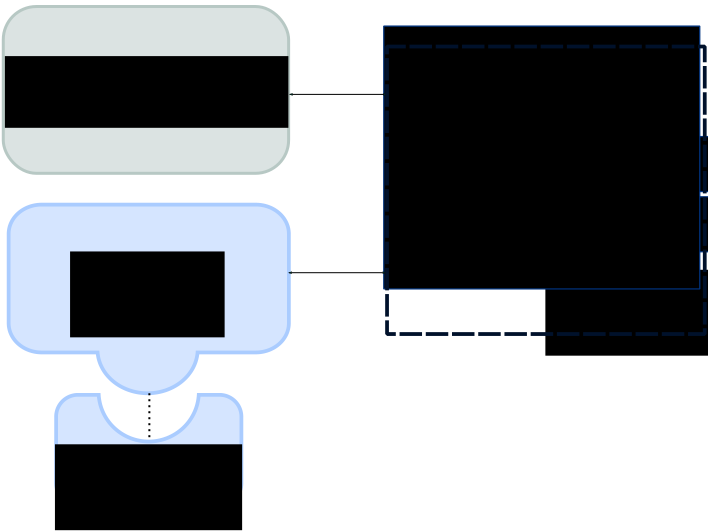
\includegraphics[scale=0.7]{figuras/metodologia1.png}
  \label{metodoetapas}
%  \legend{Fonte: autor}
\end{figure}

As características não-usuais desse sistema são listadas abaixo:

\begin{itemize}
\item Dois \textit{softwares} independentes interligados;
\item Uso de memória compartilhada para comunicação entre dois diferentes códigos;
\item Interdependência entre dados e resultados de ambos os códigos;
\item Natureza aberta das licenças de utilização de ambos os programas (item fundamental para
  o acesso, modificação e utilização do código-fonte de ambos);
\end{itemize}

Nas próximas seções serão apresentadas em seus detalhes cada uma destas características que
permitiram o desenvolvimento de um sistema multi-física.

\section{Ferramentas}
\label{sec:ferr}

O sistema acoplado desenvolvido nesta tese, utiliza dois diferentes programas de computador. Cada um deles
realiza um conjunto de cálculos separadamente e compartilham os dados necessários aos cálculos do outro.

Apesar de desenvolvidos separadamente e com objetivos diferentes, algumas características comuns - além
do fato de serem ambos \textit{software} livre - permitiram seu uso acoplado. Ambos utilizam métodos de
discretização compatíveis e possuem a capacidade de lidar com um formato aberto de arquivos de descrição
de malhas. Isso tornou possível o desenvolvimento de um acoplamento sem mapeamento, ou seja, ambos os
códigos trabalham no mesmo domínio, resolvendo suas respectivas equações no mesmo nível de detalhes
espaciais que seu oposto.

São dedicadas subseções a cada característica deste acoplamento definida anteriormente como não-usual.

\subsection{Termo-hidráulica: \textit{OpenFOAM}}
\label{subsection:openfoam}

O \textit{OpenFOAM} é um pacote orientado a objetos desenvolvido em $C++$ para simulação numérica de Mecânica
do contínuo. Do ponto de vista de Engenharia de Software, sua modularidade e flexibilidade são vantagens
em relação a outros códigos monolíticos. Sua implementação em componentes para manipulação de malhas, suporte
à solução de sistemas lineares, operadores de discretização e modelos físicos em forma de bibliotecas o tornam
um sistema CFD completo, aberto e gratuito. É utilizado em uma grande variedade
de aplicações, desde a solução de escoamentos complexos envolvendo reações químicas, turbulência e
transferência de calor até acústica, mecânica dos sólidos e eletromagnetismo. 

\textit{OpenFOAM} implementa um manipulador de malhas poliédrico, no qual células são descritas a partir
de um conjunto de faces fechando um volume. As faces, por sua vez, são formadas por uma lista de pontos
em suas coordenadas cartesianas e armazenados como vetores. Esta implementação é independente da discretização
usada \cite{Jasak2009}. Entretanto, as principais classes que herdam as funcionalidades das malhas implementam o método de
volumes finitos. Sendo assim, pode-se dizer que o \textit{OpenFOAM} é um sistema de CFD baseado em volumes
finitos.

\subsubsection{Equações}

\begin{itemize}
\item Adição do termo-fonte (1 alteração na equação do sólido: colocar equação já no formato OpenFOAM)
\end{itemize}

\subsection{Neutrônica: \textit{milonga}}
\label{subsection:milonga}

\subsubsection{Equações}

\begin{itemize}
\item Adição do termo-fonte (1 alteração na equação do sólido: colocar equação já no formato OpenFOAM)
\end{itemize}

\section{\textit{Shared-memory}}

\textit{Shared-memory} (ou memória compartilhada) é a memória de computadores que pode ser
acessada simultaneamente por múltiplos programas com o objetivo de oferecer comunicação entre
eles evitando cópias redundantes \cite{Robbins2003}. É, ainda, uma forma eficiente de passagem de dados entre programas
ou processos. A interface POSIX (\textit{Portable Operating System Interface}) é padrão especificado pela
\textit{IEEE Computer Society} para garantir a compatibilidade entre diferentes sistemas operacionais. Neste padrão
está definida uma API (\textit{Application programming interface}), ambientes de comando e cojuntos de utilitários
para compatibilidade de \textit{software} entre sistemas operacionais \cite{Atlidakis2016}.

Essa padronização permite os dois diferentes códigos usados no acoplamento utilizem-se das extensões POSIX nas
suas linguagens de programação para ler, escrever e se comunicar através do uso de memória-compartilhada.

%É desconhecido na literatura o uso de memória compartilhada (\textit{shared-memory} para
%acoplamento neutrônico e termo-hidráulico.





\section{Malha}

\begin{figure}[htb]
  \caption{Malha e regiões, vista superior.}
  \centering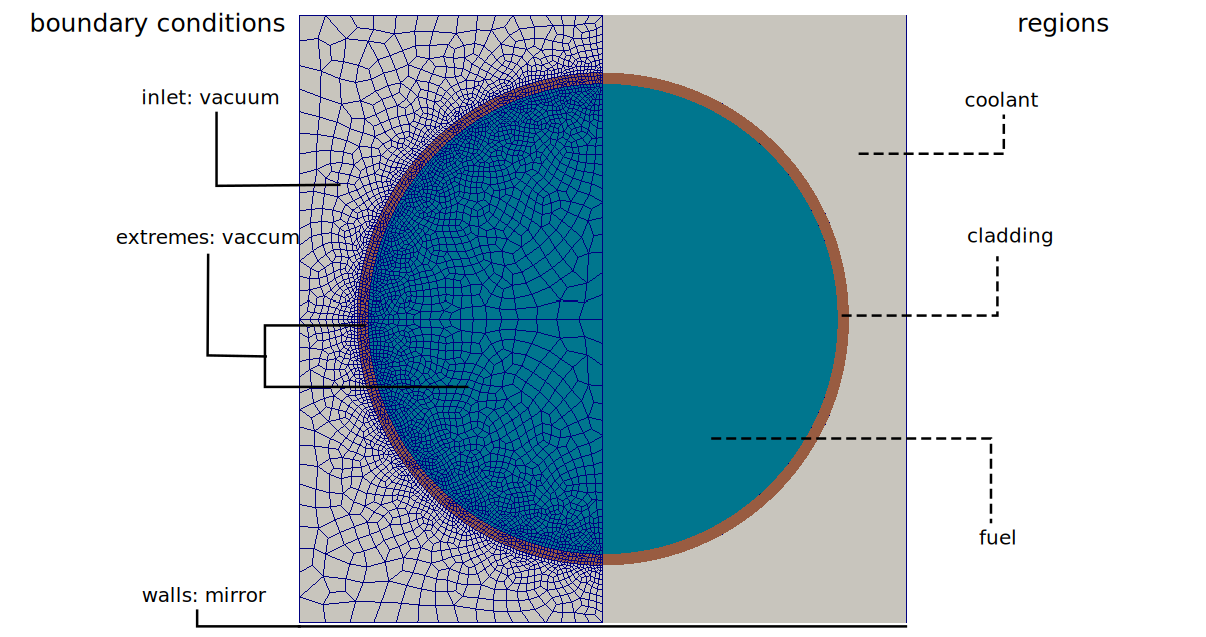
\includegraphics[scale=0.5]{figuras/regions_neutronica_malha_e_sem.png}
  \label{regions_malha}
  \legend{Fonte: autor}
\end{figure}

\section{Condições de contorno}


\section{Acoplamento} % Algoritmos

% *******************************************************************
\subsection{Estruturas de dados}

\begin{itemize}
\item Alteração de hash para vetor (1 parágrafo)
\item 1 parágrafo para a criação de Q
\item Criação de vetores shared-memory e semáforos
  \item malhas iguais
\end{itemize}

1 parágrafo: preparação para rodar em paralelo. Divisão externa ao OpenFOAM, por isso não foi
implementado. Ficou para trabalhos futuros. Até porque precisa do milonga também paralelizado.

\subsection{Algoritmo neutrônica}

\begin{figure}[htb]
  \caption{Algoritmo neutrônica.}
  \centering\includegraphics[scale=0.5]{figuras/algoritmos_milonga.png}
  \label{algo_neutronica}
  \legend{Fonte: autor}
\end{figure}

\subsection{Algoritmo termo-hidráulica}
\label{subsec:th}

\begin{figure}[htb]
  \caption{Algoritmo termo-hidráulica.}
  \centering\includegraphics[scale=0.5]{figuras/algoritmo_openfoam.png}
  \label{algo_th}
  \legend{Fonte: autor}
\end{figure}



%Modelada uma geometria idêntica à representada na malha utilizada pelo \textit{OpenFOAM},
%foram feitas simulações da neutrônica pelo Serpent com objetivo de obter as seções
%de choque em dois grupos a serem usadas na solução da aproximação por difusão dos nêutrons
%pelo \textit{milonga}.

%Na saída do Serpent são dados constantes de groups homogeneizadas (neste caso, com espectro
%corrigido para fugas pelo método B1 \textbf{CITAR}) e outros parâmetros de interesse para
%a modelagem por difusão como, por exemplo, os coeficientes de difusão para cada grupo já
%calculados.

%Como todos os elementos do desenvolvimento estão relacionados entre si, sempre que
%julgado oportuno para a clareza do entendimento, os conceitos desenvolvidos em cada
%seção poderão ser apresentados conjuntamente. De fato, uma vez que o problema multifísica
%(ou acoplamento) nada mais é do que a solução conjunta de dois problemas que são,
%usualmente, resolvidos separadamente, é natural como definir, modelar e resolver os
%dois problemas separadamente.

%De acordo com as definições de problemas acoplados apresentadas
%no capítulo \ref{chap:rev}, ao resolver os problemas neutrônico e termo-hidráulico
%separadamente, o acoplamento ainda pode ser considerado implícito de acordo com, já que a troca de informações entre os problemas ocorre ao nível de termos completos,
%e não em condições de contorno. É importante dizer que essa nomeclatura para as formas
%de acoplamento não é unânime na literatura \cite{Ivanov2007}.

%Deve estar claro que a metodologia a ser descrita trata do ciclo de desenvolvimento
%do \textit{software} acoplado. Apesar de ser possível considerar as simulações e
%os processos de pré-processamento e pós-processamento, tanto termo-hidráulicos quanto
%neutrônicos, optou-se por tratar destas etapas exclusivamente na seção de validação e,
%quando pertinente, nos resultados obtidos.


%Na figura \ref{metodoetapas} são apresentadas as relações entre os diferentes elementos
%do sistema acoplado.





